\chapter{离散随机变量}
是大$X$和小$x$,不是大S和小S。

\section*{学习目标}
\begin{todolist}
 \item 理解\gls{randomvari}是总结一个事件所有可能结果的方式
 \item 知道离散随机变量和连续随机变量,并能举出一些例子
 \item 能够根据题意求算随机变量取得特定值的概率
 \item 绘制随机变量的概率分布表
 \item 理解随机变量的\gls{expectation},并且掌握求算方法
 \item 理解随机变量的\gls{variance},并且掌握求算方法
\end{todolist}

\clearpage


\section{随机变量}
数学越往后学习,符号系统会越来越复杂。在学习求算之前,先掌握随机变量的符号。
\subsection*{标记手段和含义}
随机变量是量化一个随机事件的所有可能结果的变量,一般用大写字母表示,比如$X$或者$Y$。该变量会有不同的取值,代表随机变量的结果。

比如:\\
$X$代表扔一个骰子,骰子朝上的点数。\\
$Y$代表某医院2022.02.22出生的第一个孩子的性别\\
$Q$代表此时此刻停靠在静安寺的,往浦东机场方向的2号线列车5-4车厢里的人数\\

依次类推
\begin{TaskBox}
1. 在上面的例子当中,性别并不是一个数字。提出一种方法用数字来代表性别\\
2. 解释$P(X=3)$代表什么事情发生的概率。
\end{TaskBox}


\subsection*{随机变量的概率}
由于随机变量会有不同的取值,因此求算随机变量的概率的时候,应该分别求算每一个可取的值的时候的概率。
\begin{ExampleBox}
A fair spinner $A$ has edges numbered $1, 2, 3, 3$. A fair spinner $B$ has edges numbered $-3, -2, -1, 1$. Each spinner is spun. The number on the edge that the spinner comes to rest on is noted. Let $X$ be the sum of the numbers for the two spinners. Find the probability that $X$ is positive.
\makebox{}\hfill Adapted from 2015 winter paper6 Q6
\tcblower
$X>0$意味着$X=1$,$X=2$,$X=3$或者$X=4$。分别求算$X$取这些值的时候的概率即可。
因此有:
\[
P(X=0)=\overbrace{\frac{1}{4}}^{A=1}\times \overbrace{\frac{1}{4}}^{B=-1} + \overbrace{\frac{1}{4}}^{A=2}\times \overbrace{\frac{1}{4}}^{B=-2}+\overbrace{\frac{2}{4}}^{A=3}\times \overbrace{\frac{1}{4}}^{B=-3}
\]

依次类推,将这四种情况的概率相加即可得到$X>0$的概率
\end{ExampleBox}

\begin{SummBox}
在之前的概率求算中,基本上的标记手段为$P(A)$,现在开始采用了随机变量的$X$的形式,所以写$P(X)$并不规范。因为$X$的取值有多个,写成$P(X=x)$或者$P(X=k)$才可以计算其中取值为$x$或者$k$的概率。

因此在含有随机变量的题目当中,需要能够将$P(X=x)$翻译成语言上好理解的事件。比如$Q=100$其含义就是此时此刻停靠在静安寺的,往浦东机场方向的2号线列车5-4车厢里有100人。
\end{SummBox}

\clearpage

\section{概率分布表}
\gls{probdist}表是精炼信息的产物,是将一个随机变量的所有结果以及对应的概率进行的汇总表格。一般而言会有两行,第一行填入任意随机变量的取值;第二行的对应位置填写该随机变量的概率。
如下图所示:
\begin{figure}[H]
\centering
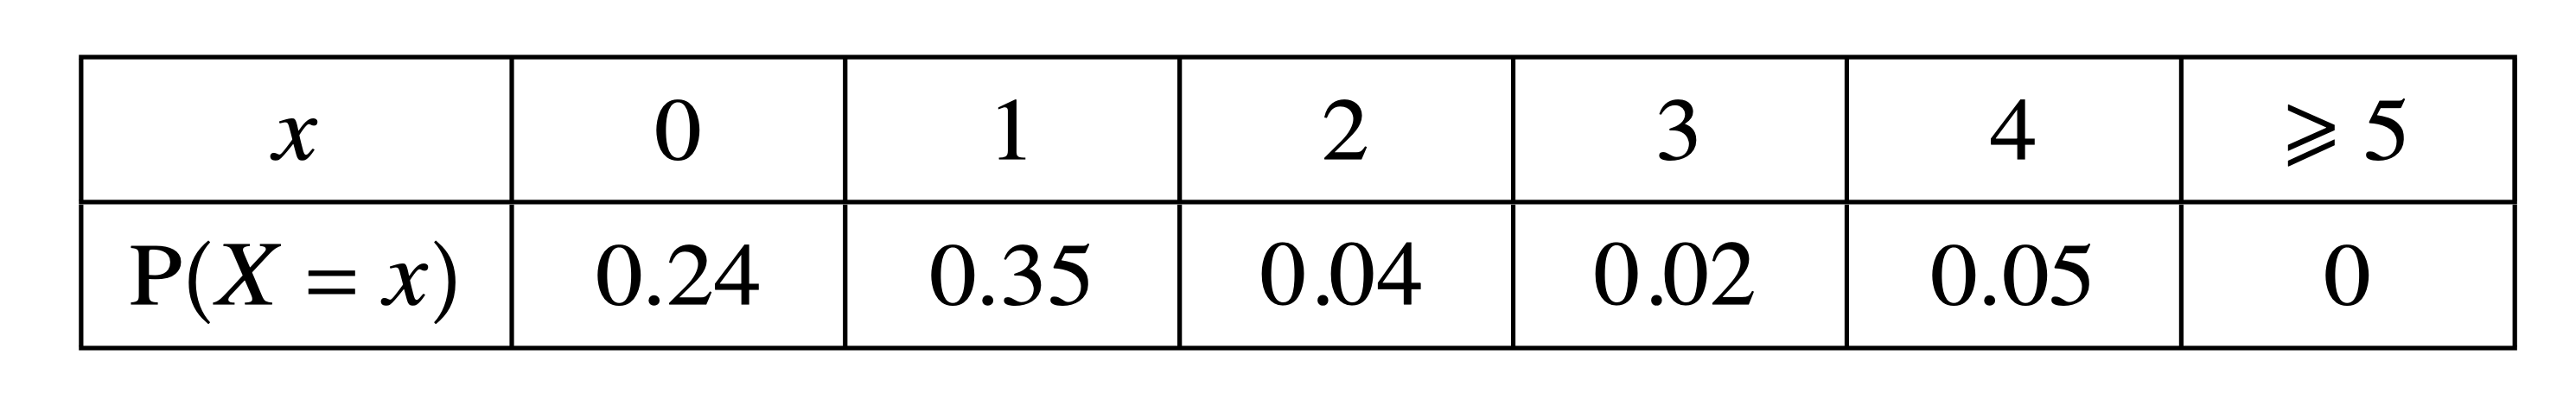
\includegraphics[width=0.5\textwidth]{probability table.png}
\end{figure}

\subsection*{概率分布表的性质}
\label{subsec:property}
由于随机变量的概率分布表是把所有的可能结果以及概率都列出来的,因此根据之前所学的全概率公式,这些概率相加只和为1,这是概率分布表最为重要的性质,也是考试经常会出的考点之一。

用求和符号的写法为:
\[
	\sum_{x_{min}}^{x_{max}} P(X=x)=1
\]

\clearpage

\section{期望与方差}
在确定了一个随机变量的分布情况之后,还可以去研究一个随机变量的期望和方差。
\subsection*{期望}
\label{subsec:Expectation}
\gls{expectation}实际上来自于非常著名的\href{https://mp.weixin.qq.com/s/5XVSg-MaZYsaiM2agwHpLA}{分赌注问题}。最后由帕斯卡,费马,还有惠更斯三人顺利解决。感兴趣的可以点击超链接了解详情。是概率当中最为重要的一环,同时也是概率论这一门学科的起源。其正式定义为:随机变量的取值的加权平均数,权重为该取值发生的概率。计算公式较为简单,如下:
\[
	E(X)/\mu=\sum x_i\cdot P(x_i)
\]
其中$x_i$是取值,$P(X=x_i)$是概率。

\begin{ExampleBox}
如何理解期望才是一个难点。虽然考试基本上的形式以计算为主,但是能够对期望这个概率论的起源有个较为深刻的理解必定能够助力学好概率论。
\tcblower
以抛硬币为例,如果正面朝上就能获得一块钱,反面朝上没有钱。但是参加这个游戏需要支付$0.6$(话说,你们觉得那一面是正面?)随机变量$X$记录玩一次的收益,那么$X$的分布就是很简单的\gls{0-1distr}。分别有$X=0$ 概率为$1/2$;$X=1$ 概率为$1/2$。那么玩一次这样的游戏,收益的\textbf{期望}就是$0.5$。但是随机变量$X$要么是1,要么是0。不可能出现为0.5的结果。

所以应该从这个角度理解:重复这个随机试验10000次,由于之前的概率分布,假设在非常理想的情况下,10000次当中会有5000次正面朝上,意味着可以收获到5000元,但是也会有5000次反面朝上,意味着颗粒无收。所以,总共平均到每一次游戏的\textbf{平均收益}就是0.5

对比一下两个0.5产生的过程
\begin{matrix}
 0.5=0\times \frac{1}{2}+1\times\frac{1}{2} & 0.5=\frac{0\times 5000+1\times5000}{10000}
\end{matrix}
不难发现,概率当中的期望实际上就是重复做这个随机试验,得到的平均值。不过在这里有一个前提,就是10000次当中有50000次朝上,5000次朝下。但是如果真的有人去做这个10000次的实验的话,不一定刚好这么\textbf{理想}。因此我们再加上一个限制条件,重复做这个实验\textbf{无限多次}。这样就能够确保,正面朝上的\emph{频率}一定等同于它的\emph{理论概率}。从这个角度理解期望就比较容易了。

那么,站在一个理性人角度出发,是否应该去玩这个游戏?
\end{ExampleBox}

\subsection*{方差}
这里的\gls{variance}的概念和之前统计学当中的方差的概念是完全一致的,只不过是将原公式当中的频率$f$替换为概率$P$。代表着随机变量的波动程度。

定义公式如下:
\[
	Var(X)/\sigma^2 = \sum (x_i-\mu)^2\cdot P(x_i)
\]

经过化简之后的计算公式如下:
\[
	Var(X)/\sigma^2 = \left(\sum x_i^2\cdot P(x_i)\right)-\mu^2
\]


\begin{ExampleBox}
The discrete random variable $Q$ is such that $Q\quad \in \{1,2,3,5\}$ and $P(Q=q)=\frac{1}{2}-kq$ where $k$ is a constant.
\begin{itemize}
\item
Show that $k=\frac{1}{11}$
\item
Calculate the expectation and variance of $Q$
\end{itemize}

\tcblower
为了方便,可以列出$Q$的概率分布表。如下
\begin{table}[H]
\centering
\begin{tabular}{|l|c|c|c|c|}
\hline
$q$      & 1                      & 2                      & 3                      & 5                      \\ \hline
$P(Q=q)$ & $\frac{1}{2}-1\cdot k$ & $\frac{1}{2}-2\cdot k$ & $\frac{1}{2}-3\cdot k$ & $\frac{1}{2}-5\cdot k$ \\ \hline
\end{tabular}
\end{table}

因此可以利用\ref{subsec:property}将所有的概率全部累加,永远等于$1$。得到
\[
4\times \frac{1}{2} - 11k = 1 \quad \Longrightarrow  \quad k =\frac{1}{11}
\]

该随机变量的概率分布表为
\begin{table}[H]
\centering
\begin{tabular}{|l|c|c|c|c|}
\hline
$q$      & 1                      & 2                      & 3                      & 5                      \\ \hline
$P(Q=q)$ & $\frac{9}{22}$ & $\frac{7}{22}$ & $\frac{5}{22}$ & $\frac{1}{22}$ \\ \hline
\end{tabular}
\end{table}
用该表去求算期望的公式为:
\[
	E(Q)= \sum x_i\cdot p_i =1\cdot \frac{9}{22}+2\cdot \frac{7}{22}+3\cdot \frac{5}{22}+5\cdot \frac{1}{22} = \frac{43}{22}
\]

用该表去求算方差的公式为:
\[
	Var(Q)=\sum x_i^2\cdot p_i-E(Q)^2=1^2\cdot \frac{9}{22}+2^2\cdot \frac{7}{22}+3^2\cdot \frac{5}{22}+5^2\cdot \frac{1}{22}-(\frac{43}{22})^2 =\frac{505}{484}
\]
\end{ExampleBox}


\subsection*{标准差}
那么标准差和统计学当中的一样,也是随机变量方差正的平方根。
\[
	\sigma = \sqrt{Var(X)}
\]

不过一般在涉及概率分布的考题当中,一般求算到方差就可以了,不太会考察标准差。

\begin{SummBox}
1. 概率分布表的全部概率之和为1\\
2. 求算期望的公式是$E(X)/\mu = \sum x_i\cdot P_i$\\
3. 再计算完随机变量的期望之后,才可以求算该随机变量的方差,公式为$\sum x_i^2\cdot P_i - E^2(X)$
\end{SummBox}








